\documentclass[11pt]{article}

\usepackage[utf8]{inputenc}
\usepackage[english]{babel}

\usepackage{hyperref}     % For \autoref
\usepackage{parskip}      % Don't indent paragraphs; skip instead.

\usepackage{amsfonts, amsmath, amssymb}
\usepackage{amsthm}
\usepackage{changepage}   % For adjustwidth environment
\usepackage{colortbl}     % Provides the  \arrayrulecolor command.
\usepackage{environ}
\usepackage{framed}       % For leftbar environment
\usepackage{mathtools}    % For the \mathclap command.
\usepackage{ragged2e}     % FlushLeft environment
\usepackage{thmtools}     % For restatable environment
\usepackage{varwidth}
\usepackage{xcolor}
\usepackage{makeidx}
\usepackage{bm}           % For vector bold
\usepackage[margin=3cm]{geometry}


\newenvironment{indentone}{\begin{adjustwidth}{3em}{0em}}{\end{adjustwidth}}

% \renewcommand{\bfseries}{\scshape}
% \usepackage{ccfonts}
\newcommand\op[1]{{\ \mathrm{#1}\ }}
\newcommand\uop[1]{{\mathrm{#1}}}

\newcommand\AND{{\op{AND}}}
\newcommand\IMPLIES{{\op{IMPLIES}}}
\newcommand\MYS{{\op{MYS}}}
\newcommand\OR{{\op{OR}}}
\newcommand\NOT{{\uop{NOT}}}
\newcommand\XOR{{\op{XOR}}}
\newcommand\IFF{{\op{IFF}}}
\newcommand\VEC{\bm}{}
\newcommand\DIV{\>|\>}

\newcommand\FALSE{{\mathrm{F}}}
\newcommand\TRUE{{\mathrm{T}}}

% Number sets
\newcommand{\Nats}{\mathbb N}   % Naturals
\newcommand{\Ints}{\mathbb Z}   % Integers
\newcommand{\Q}{\mathbb Q}      % Rationals
\newcommand{\R}{\mathbb R}      % Reals
\newcommand{\C}{\mathbb C}      % Complexes
\newcommand{\cO}{\mathcal O}    % Big-Oh
\newcommand{\cP}{\mathcal P}    % Power set

\theoremstyle{definition}
\newtheorem{theorem}{Theorem}[section]
\newtheorem{corollary}{Corollary}[section]
\newtheorem{lemma}{Lemma}[section]
\newtheorem{proposition}{Proposition}[section]
\newtheorem{definition}{Definition}[section]
\newtheorem{remark}{Remark}[section]
\newtheorem{example}{Example}[section]
\newtheorem{question}{Question}[section]
\newtheorem{problem}{Problem}[section]
\newtheorem{exercise}{Exercise}[section]
\newtheorem{homework}{Homework}[section]
\newtheorem{algorithm}{algorithm}[section]
\numberwithin{equation}{section}
% \newtheorem*{corollary}{Corollary}
% \newtheorem*{theorem}{Theorem}
% \newtheorem*{definition}{Definition}
% \newtheorem*{remark}{Remark}


% Essential sections of notes, e.g. definitions/theorems.
\NewEnviron{bigbox}{{

    \newdimen\slidewidth
    \slidewidth=\linewidth
    % Without this, I get errors beginning "Overfull \hbox (6.79999pt too
    % wide)"
    \advance\slidewidth by -7pt

    \medskip

    \fbox{parbox{\slidewidth}{\BODY}}

    \medskip

  }}

% Stuff I should write or draw during lecture. (from James)
% Additional notes
\NewEnviron{writenotes}{\vspace{1ex}\begin{leftbar}{\BODY}\end{leftbar}}


\title{Notes\\
  {\large STA314H1 - Fall 2020}}
\author{Ziyue Yang}

\begin{document}
\maketitle

\tableofcontents

\newpage

\section{Week 5}

\subsection{Norms}

\subsubsection{Induced Norm of a Matrix}

\begin{question}
  If we have a vector $x$ and a matrix $A$, how big is $Ax$ compared to $x$?

  Suppose that we find a constant $C_{A, q}$ such that
  \begin{equation}
    \| Ax\|_q \leq C_{A, q}\|x\|_q,
  \end{equation}
  then the \textbf{smallest such constant} would be a good indication of how much multiplying by $A$ changes the length of a vector.
\end{question}
\begin{writenotes}
  This lets us define the \textbf{induced norm} of a matrix
\end{writenotes}

\begin{definition}[The Induced Norm of a Matrix]
The induced norm of a matrix $A$ is defined as
  \begin{equation}
    \|A\|_q = \sup_x\frac{\|Ax\|_q}{\|x\|_q}.
  \end{equation}
\end{definition}

\begin{writenotes}
  NB: This works when $A$ is rectangular.
\end{writenotes}

\subsubsection{jj2-Norm of a Matrix}

We hold a special place for 2-norms, as well as the induced 2-norm of a matrix.

\begin{definition}[The Induced 2-Norm of a Matrix]
  \begin{equation}
    \|A\|_2^2 = \sup_x\frac{\|Ax\|^2_2}{\|x\|^2_2}=\sup_x\frac{x^TA^TAx}{x^Tx}.
  \end{equation}
  Note that this is the \textbf{largest eigenvalue of} $A^TA$. Hence the 2-norm of a matrix $A$ is the square root of the largest eigenvalue of $A^TA$.
\end{definition}

\subsubsection{Orthogonal Invariance} 
It turns out that both the matrix and vector 2-norms are invariant to multiplication by an orthogonal matrix. Note that this is NOT true for other norms.

\begin{example}
Suppose $U$ is a $p\times p$ orthogonal matrix, then

\begin{equation}
 \|Ux\|^2_2=x^TY^TYx=x^Tx=\|x\|^2_2.
\end{equation}
  Suppose $A$ is an $n\times p$ matrix, $V$ is an $n\times n$ orthogonal matrix. Then
  \begin{equation}
    \|U^TAVx\|^2_2=\|U^TA\tilde{x}\|^2_2=\tilde{x}^TA^TUU^TA\tilde{x}=\tilde{x}^TA^TA\tilde{x},
  \end{equation}
  where $\tilde{x}=Vx, \|\tilde{x}\|^2_2=\|x\|_2$ and so
  \begin{equation}
    \|U^TAV\|_2=\|A\|_2.
  \end{equation}

\end{example}


\subsection{The Singular Value Decomposition (of Non-Symmetic and Rectangular Matrices)}

\begin{remark}
 We know that $\| X \|_2$ is the square root of the largest eigenvalue of $X^T X$, hence at some point , whenever we see one of the inner product matrices, we should recall the \textbf{PCA}.

 The SVD is a good way to understand exactly how PCA is working in terms of the feature matrix $X$.
\end{remark}

\begin{theorem}[The Singular Value Decomposition]
  Assume that $p < n$.

  Let $X$ be an $n\times p$ matrix. Then there exists an orthogonal $p\times p$ matrix $V$ (i.e. $V^T V = VV^T = I$) and an orthogonal $n\times n$ matrix $U$ such that
  \begin{equation}
    U^TXV=D,
  \end{equation}
where $D=\text{diag}(\sigma_1,\dots,\sigma_p)$, and $\sigma_1\geq \dots\geq \sigma_p\geq 0$.
\end{theorem}

\begin{proof}
  Omitted for now.
\end{proof}

\subsubsection{The SVD and Principal Components}

\begin{remark}
  So what good is an SVD? 

  The SVD is like the \textit{eigendecomposition} of a symmetic matrix, except it is defined for \textbf{all} matrices.

  We can express the SVD of an $n\times p$ matrix $X$ in several equivalent ways:
  \begin{enumerate}
    \item As a singular tuple $(\sigma,u,v)$ that satisfies $Xv=\sigma u$ and $X^Tu=\sigma v$.
    \item As a matrix decomposition $X=UDV^T$, where $V$ is a $p\times p$ orthogonal matrix, and $U$ is a $n\times n$ orthogonal matrix.
    \item As a way of representing the matrix as a sum
    \begin{equation}
      X=\sum^p_{j=1}\sigma_j u_j v_j^T.
    \end{equation}
  \end{enumerate}
\end{remark}

\begin{remark}[The SVD and Principal Components]
 Recall that the factor loadings are the eigenvectors of $X^TX$.

 If $X=UDV^T$, then $X^TX=V^TDU^TUDV^T=VD^2V^T$.
 \begin{itemize}
 \item The $V$ in the SVD is exactly the matrix of factor loadings.
 \item The eigenvalues of $X^TX$ are the squares of the singular values.
 \end{itemize}
 Note that the score vectors were defined as $t_j=Xv_j$, and We can use one of the representations of singular vectors to see that
 \begin{equation}
   t_j=Xv_j=\sigma_j u_j.
 \end{equation}
\end{remark}

\subsubsection{SVD and Principlal Component Regression}
\begin{remark}
  The SVD makes it easy to solve the normal equations.

  Recall that
  \begin{align}
    \hat\beta &= (X^TX)^{-1}X^Ty\\
    &=VD^{-2}V^TVDU^Ty\\
    &=VD^{-1}U^Ty\\
    &=\sum^p_{j=1}\frac{u_j^T y}{\sigma_j}v_j.
  \end{align}

  PCR just snipes off the small eigenvectors:
  \begin{equation}
    \hat\beta_{\text{pcr}}=V_kD_k^{-2}V_k^TVDU^T=\sum^k_{j=1}\frac{u_j^Ty}{\sigma_j}v_j.
  \end{equation}
\end{remark}

\subsection{Ridge Regression}

\subsubsection{Overfitting Discussion}

As we add more features to our regression, our training error will decrease, as our test error will go down for a while, then will increase again. A sign that something has gone wrong is that we have wildly varying regression coefficients, reasons include
\begin{itemize}
  \item (Almost) co-linearity of features;
  \item Big feature weights are needed to fit data perfectly,
\end{itemize}

which can lead to out-of-sample \textit{bias}.

\textbf{What if we force the coefficients to be small?}

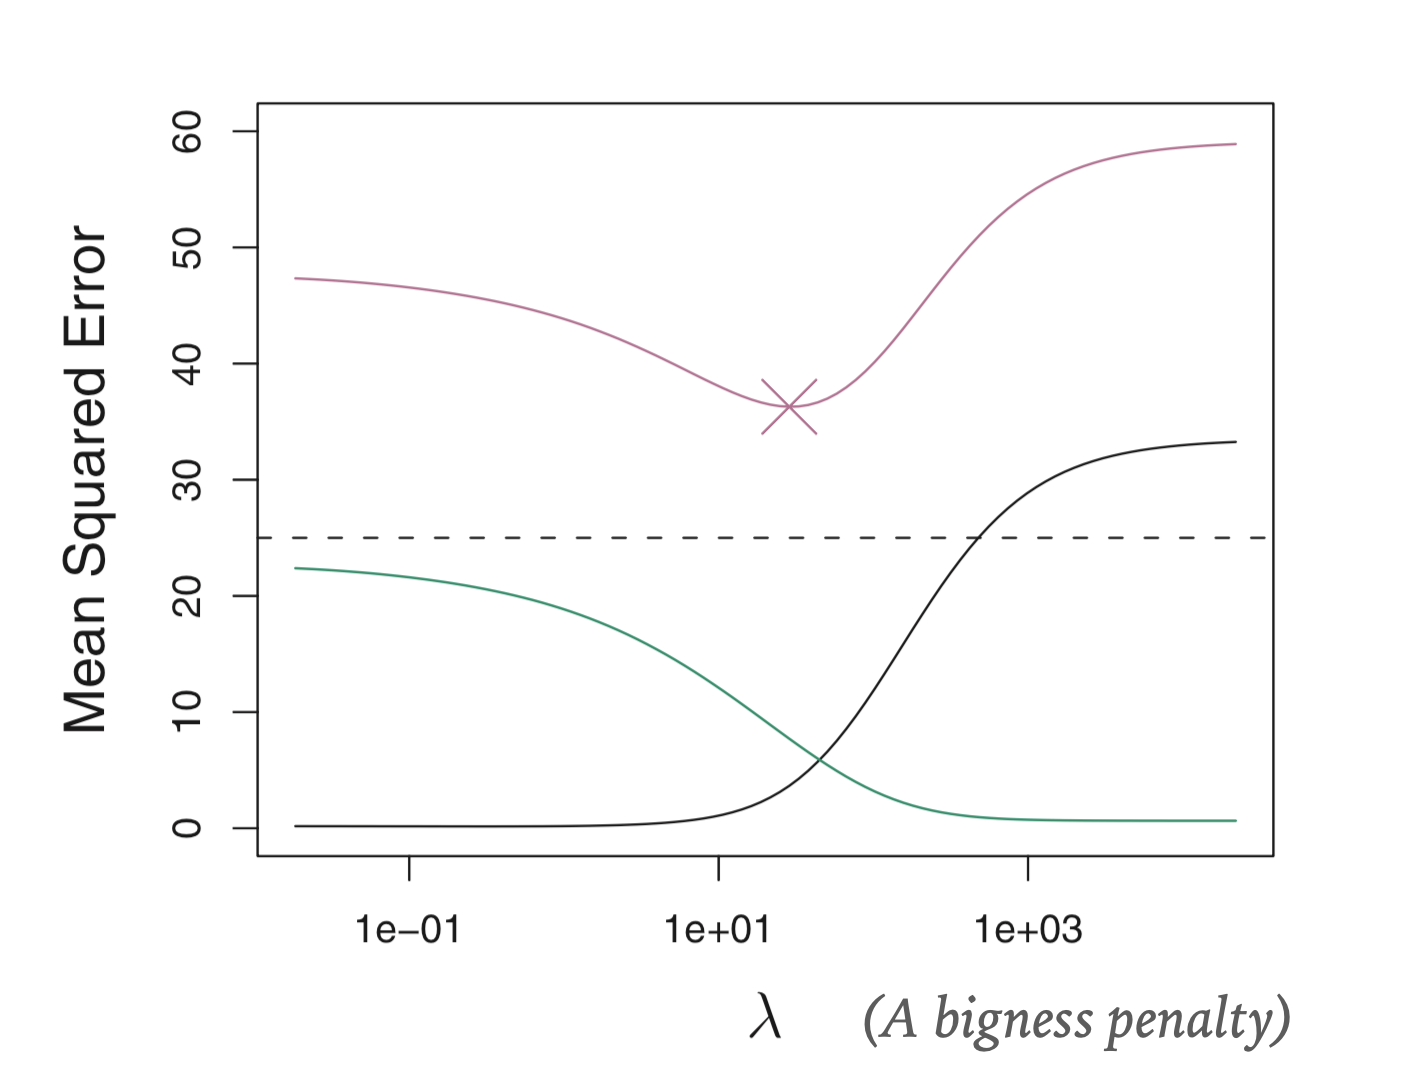
\includegraphics[scale=0.4]{./images/overfitting.png}

\textbf{The idea is:} \textit{Don't let things get to big}.

\subsubsection{Ridge Regression Objective Function}

Instead of solving our standard least-squares problem, we should use the \textbf{ridge regression} objective function.

\begin{definition}[Ridge Regression Objective Function]
\begin{equation}\label{ridge-objective}
  \min_{\beta_0, \beta}\sum^n_{i=1}(y_i-\beta_0-X\beta)^2 + \lambda\|\beta\|^2_2.
\end{equation}
\end{definition}

This means that we need to \textbf{balance} the goodness of fit with the requirements that the $\beta_j$ aren'r too big. The parameter $\lambda$ controls the balance. 
\begin{indentone}
If $\lambda = 0$, we recover LS;

If $\lambda\to\infty$, then all the coefficeints are zero.
\end{indentone}
\begin{writenotes}
  Side note about the intercept...

  If we want to include an intercept term, it's importatnt to make sure the features are \textbf{centred}, in which we can do quick maths to show that the first row of the normal equation is
  \begin{equation}
    1^T
    \begin{pmatrix}
      1&X
    \end{pmatrix}
    \begin{pmatrix}
      \beta_0\\
      \beta
    \end{pmatrix}
    =1^Ty.
  \end{equation}
  If $X$ is centred (such that $1^TX=0$), then it follows that
  \begin{equation}
    \beta_0=\frac{1}{n} \sum^n_{i=1}y_i
  \end{equation}
  \textit{Points to $y_i$: don't shirnk.}
\end{writenotes}

\textbf{What does the solution look like?}

Assuming we cetre the predictors, we already know what the value of $\beta_0$ is. Now assume that the data has the mean of zero. Notice that the objective function (\ref{ridge-objective}) is \textit{smooth} and quadratic, so we can minimize it as before.

The components of the gradient are
\begin{align}
  \frac{\partial}{\partial\beta_k}\left[ \sum^n_{i=1}\left( y_i-\sum^p_{j=1}\beta_jx_{ij} \right)^2+\lambda\sum^p_{j=1}\beta_j^2 \right]
  &=2\sum^n_{i=1}\left( y_i-\sum^p_{j=1}\beta_jx_{ij} \right)x_{ik}+2\lambda\beta_k\\
  &=2X^Ty-2X^TX\beta-\lambda\beta\\
  &=0\qquad\text{when }(X^TX+\lambda I)\beta=X^Ty.
\end{align}

\subsubsection{Ridge Regression Estimates}
By performing a \textbf{singular value decomposition} of $X$, we obtain
\begin{equation}
  X=UDV^T,
\end{equation}
here
\begin{indentone}
  $U$ and $V$ have orthonormal columns,

  $D$ is diagonal
\end{indentone}

This is related to the eigendecomposition by
\begin{equation}
  X^TX=VDU^TUDV^T=VD^2V^T,
\end{equation}
plugging which into the ridge regression equations (?ref here), we get
\begin{align}
  (X^TX+\lambda I)\beta&=X^Ty\\
  V(D^2+\lambda I)V^T\beta&=VDU^Ty\\
  V^T\beta&=(D^2+\lambda I)^{-1}DU^Ty\\
  \beta&=V(D^2+\lambda I)^{-1}DU^Ty.
\end{align}

\textbf{What does the fit look like?}

Comparison of $\beta_{ridge}$ and $\beta_{LS}$:

\begin{gather}
  \beta_{bridge}=\sum^p_{j=1}\frac{\sigma_j}{\sigma_j^2+\lambda}v_ju_j^Ty\\
  \beta_{LS}=\sum^p_{j=1}\frac{1}{\sigma_j}v_ju_j^Ty
\end{gather}

Hence the ridge regression shrinks each coefficient by a factor of
\begin{equation}
  \frac{\sigma^2_i}{\sigma^2_i+\lambda}.
\end{equation}
\begin{writenotes}
  Note that the shrinkage is NOT uniform.

  Refers to \textit{Week 5, Part 3: Ridge Regression}.
\end{writenotes}


\section{Week 6 (Quiz 1)}

\newpage

\section{Week 7}
\subsection{Introduction to Lasso}

\begin{remark}
  Ridge regression stabilizes the least-squares estimates by shrinking low-variance directions, which makes it like a \textit{softer} version of \textbf{principal component regression}.
\end{remark}

\begin{writenotes}
  Can we use penalized regression to make a softer version of variable selection? Yes. But we need to use a different penalty.
\end{writenotes}

\textbf{OMITTED TO SAVE TIME}

\section{Week 8/9}
% Part 4
\subsection{Logistic Regression}
% Skipped basic concepts
\subsubsection{Classification Boundaries}

 From the Bayes' classifier we know that the best decision boundary is $Pr(y=1\>|\>x)=0.5$.

 Taking logs, we observe that
 \begin{gather}
   \log(Pr(y=1\>|\> x))= -\log 2\\
   \log(1 - Pr(y=1\>|\> x))= -\log 2
 \end{gather}
 implying that the decision boundary is
 \begin{equation}
   \implies\log\left( \frac{Pr(y=1\>|\> x)}{1 - Pr(y=1\>|\> x)} \right)=\beta_0+x^T\beta=0.
 \end{equation}
\begin{writenotes}
  This is a linear boundary.
\end{writenotes}

\subsubsection{Separation and Remedies}

% ... separation stuff
% begin with penalty
\textbf{Separation} \textit{occasionally/almost} happens with real data, especially when there are a lot of predictors.

An option to prevent this is to add a penalty, which prevents us from being able to increase the value of $\beta$ forever.

\begin{indent}
  L1-penalized logistic regression/logistic lasso minimizes
  \begin{equation}
  -\frac{1}{n}\sum^n_{i=1}(y_i\log(p(\beta,x_i)) + (1-y)\log(1-p(\beta, x_i))) + \lambda\| \beta \|_1
  \end{equation}

  L2-penalized logistic regression minimizes
  \begin{equation}
  -\frac{1}{n}\sum^n_{i=1}(y_i\log(p(\beta,x_i)) + (1-y)\log(1-p(\beta, x_i))) + \lambda\| \beta \|^2_2
  \end{equation}
\end{indent}

\end{document}